\section{Adapter Tuning}
Adapter tuning \citep{NIPS2017_e7b24b11} inserts small modules called \defn{adapters} \index{adapter} to a model. Adapters can be any network architectures and can be placed anywhere in the model, but many follow \citet{pmlr-v97-houlsby19a}'s practice to place a two-layer feed-foward neural network with a bottleneck after each sublayer (including both the multi-head attention sublayer and the feed-forward sublayer) within the transformer (\cref{fig:adapter}):  
\begin{equation}
    \textbf{h}\leftarrow \textbf{h}+f(\textbf{h}\textbf{W}_{\text{down}})\textbf{W}_{\text{up}}
\end{equation}
where $f$ is a nonlinear activation function.

% \begin{figure}[htbp]
%     \floatbox[{\capbeside\thisfloatsetup{capbesideposition={right,top},capbesidewidth=4cm}}]{figure}[\FBwidth]
% {\caption{A test figure with its caption side by side}\label{fig:test}}
% {
%     \begin{subfigure}[t]{0.24\textwidth}
%          \centering
%          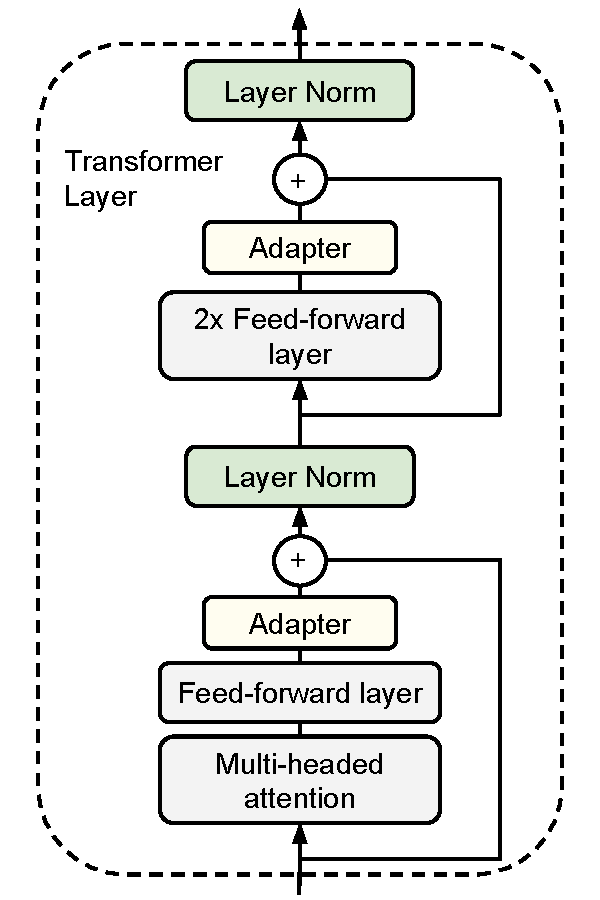
\includegraphics[width=\textwidth]{figures/parameter_efficient_finetuning/Adapter_insertion.pdf}
%          \caption{Adapters are inserted after the multi-head attention sublayer and the feed-forward sublayer.}
%     \end{subfigure}
%     \hfill
%     \begin{subfigure}[t]{0.24\textwidth}
%          \centering
%          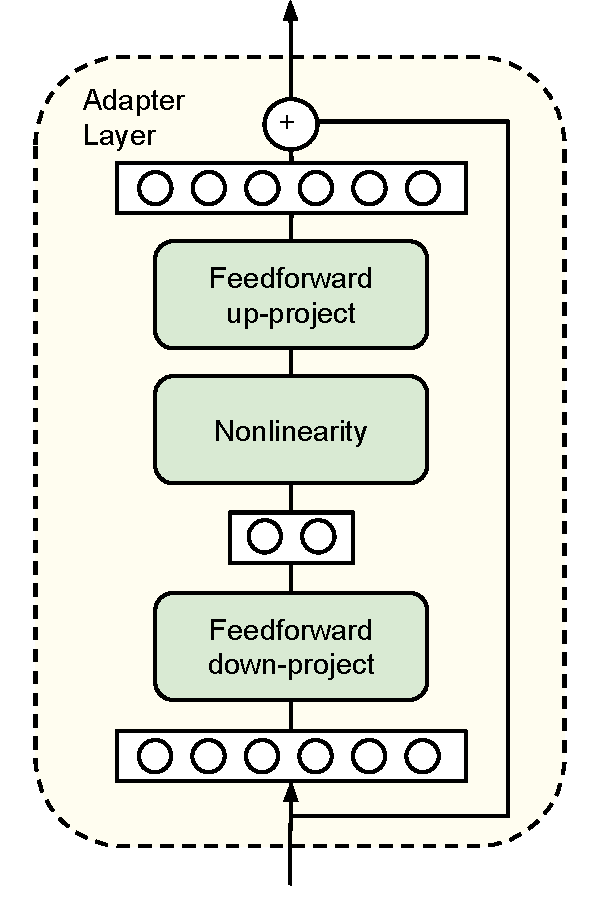
\includegraphics[width=\textwidth]{figures/parameter_efficient_finetuning/Adapter_arch.pdf}
%          \caption{The adapter consists of a down-projection, an up-projection, and a skip-connection. The intermediate hidden state typically have smaller size, which is thereby called a "bottleneck".}
%     \end{subfigure}
%     \caption{Adapter \cite{pmlr-v97-houlsby19a}. During adapter tuning, blocks in green are trained, including adapters, layer normalizations, and the final classification layer (not shown in the figure).}
%     \label{fig:adapter}
%     }
% \end{figure}

\begin{figure*}
    \centering
 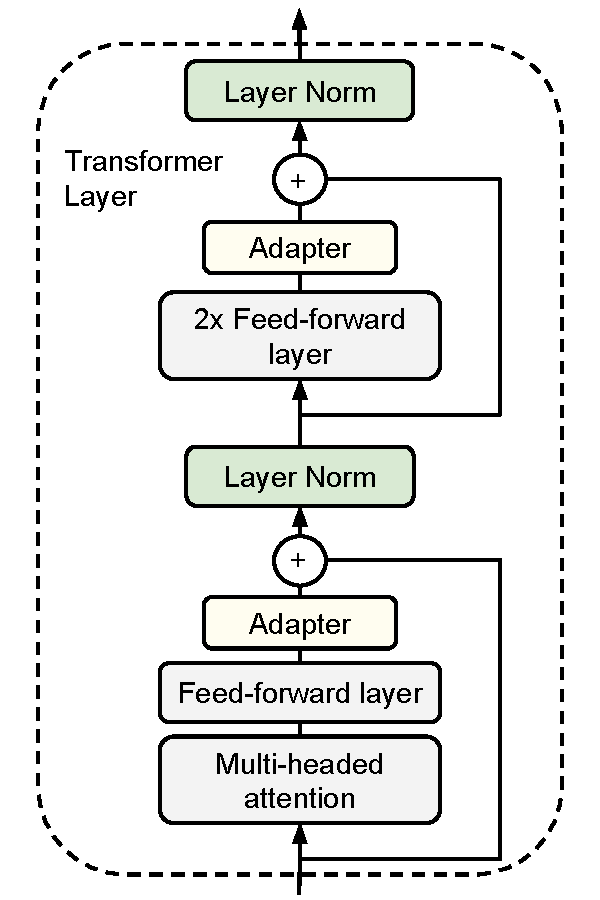
\includegraphics[width=0.3\linewidth]{figures/parameter_efficient_finetuning/Adapter_insertion.pdf}
 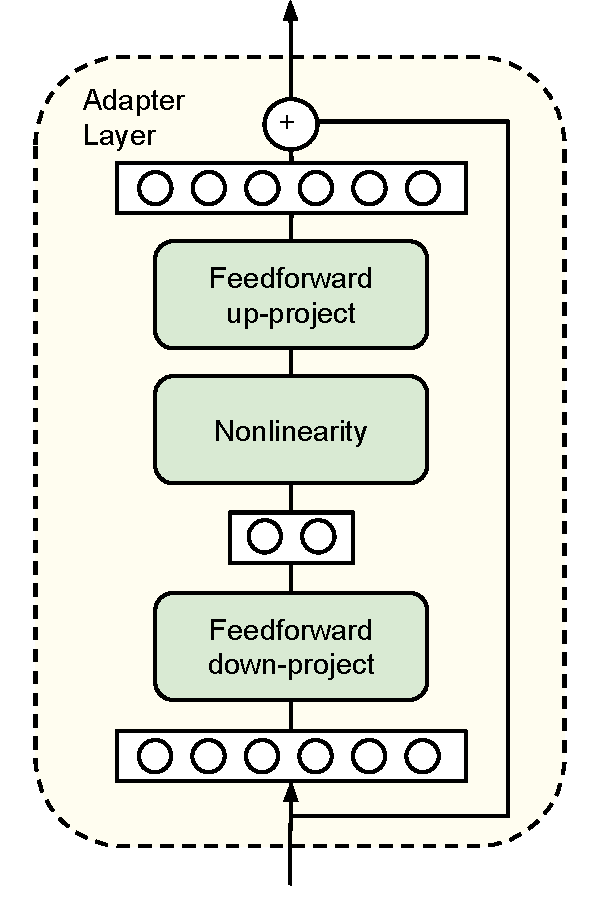
\includegraphics[width=0.3\linewidth]{figures/parameter_efficient_finetuning/Adapter_arch.pdf}
    % \begin{subfigure}[t]{0.3\textwidth}
    %      \centering
    %      \caption{}
    % \end{subfigure}
    % \hfill
    % \begin{subfigure}[t]{0.3\textwidth}
    %      \centering
    %      \caption{The adapter consists of a down-projection, an up-projection, and a skip-connection. The intermediate hidden state typically have smaller size, which is thereby called a "bottleneck".}
    % \end{subfigure}
 \caption{
Left: Adapters are inserted after the multi-head attention sublayer and the feed-forward sublayer.
Right: The adapter consists of a down-projection, an up-projection, and a skip-connection. The intermediate hidden state typically have smaller size, which is thereby called a ``bottleneck''.
Taken from \citet{pmlr-v97-houlsby19a}.
During adapter tuning, blocks in green are trained, including adapters, layer normalizations, and the final classification layer (not shown in the figure).
 \label{fig:adapter}}
\end{figure*}

It has been shown that adapter tuning can attain performance comparable to full fine-tuning by training only a small fraction of parameters (\cref{fig:adapter_results}). 

\begin{figure}
    \centering
    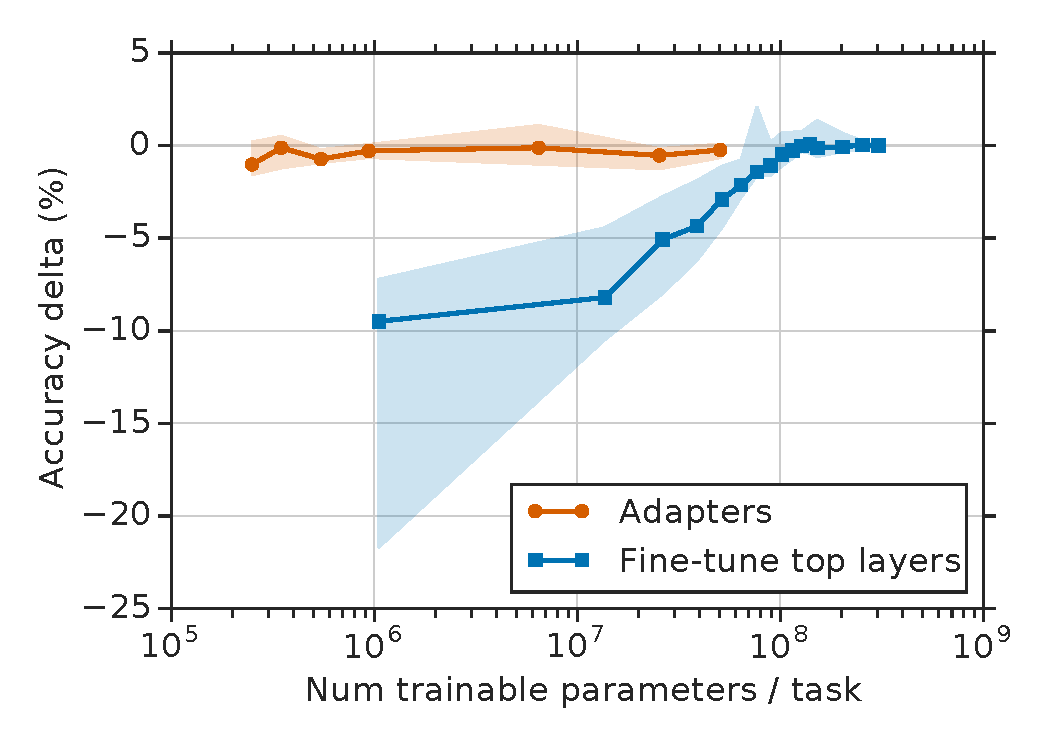
\includegraphics[width=0.6\textwidth]{figures/parameter_efficient_finetuning/glue_results_b.pdf}
    \caption{Number of trained task-specific parameters for adapter tuning and fine-tuning.}
    \label{fig:adapter_results}
\end{figure}

\subsection{Example: Cross-Lingual Transfer [Optional]}
In this section, we introduce the application of adapters to cross-lingual transfer. LLMs pretrained on multiple languages such as multilingual BERT \citep{devlin-etal-2019-bert} and XLM-R \citep{NEURIPS2019_c04c19c2} enables few-shot or even zero-shot cross-lingual transfer to low-resource languages \citep{pires-etal-2019-multilingual}. However, the capacity of a single model is limited: it cannot cover an unlimited number of languages and better performance on low-resource languages often comes at the cost of worse performance on high-resource languages (compared to monolingual models) \citep{conneau-etal-2020-unsupervised}. To alleviate the issue, we can learn an adapter for each language, which allows the model to incorporate more languages without having the languages interfering with each other. 

\citet{pfeiffer-etal-2020-mad} proposed the Multiple ADapters for Cross-lingual transfer (MAD-X) framework (\cref{fig:madx}), which comprises three types of adapters: language, task, and invertible adapters.

\begin{figure}
    \centering
    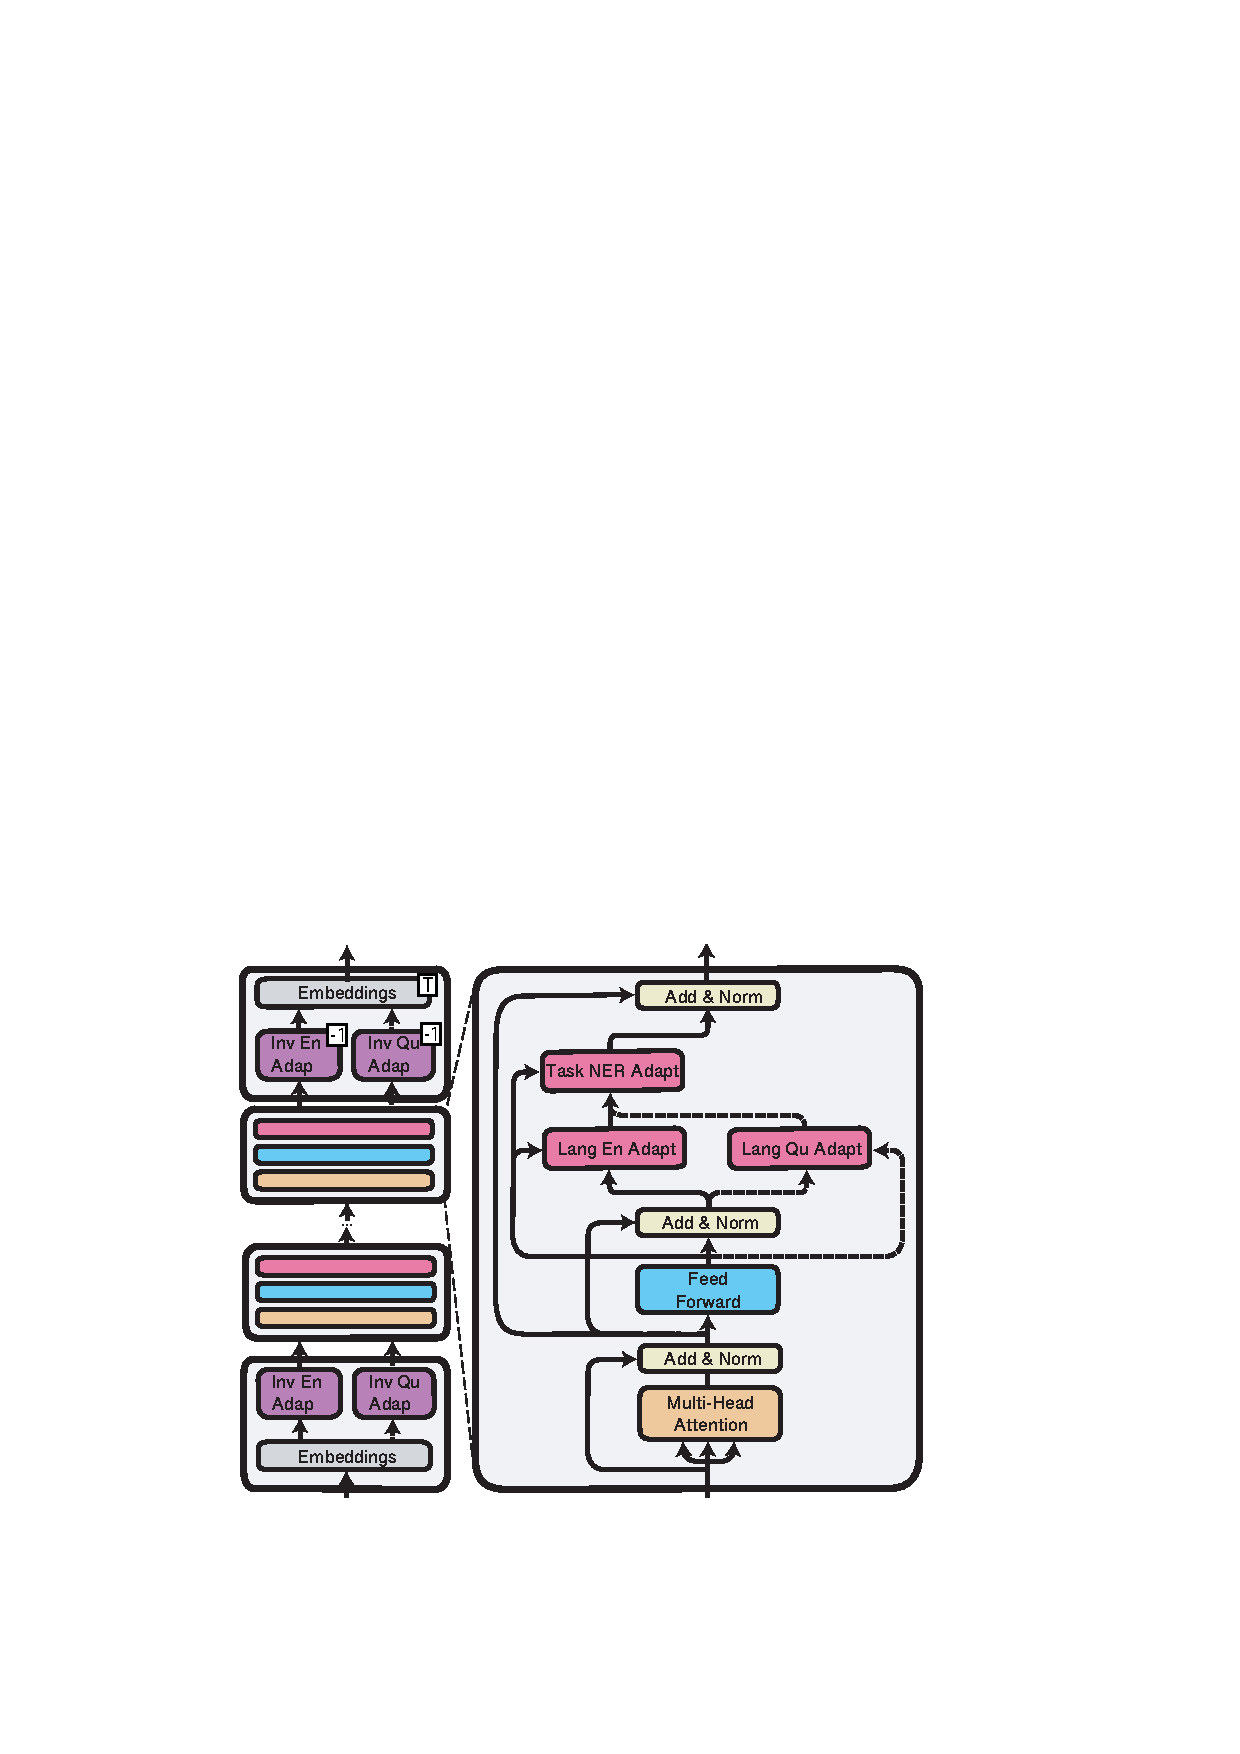
\includegraphics[width=0.6\textwidth]{figures/parameter_efficient_finetuning/MAD-X_combined.pdf}
    \caption{Diagram of the MAD-X framework showing the integration of language-specific, task-specific, and invertible adapters within a transformer-based model architecture. Language adapters and invertible adapters are incorporated into every layer of the Transformer architecture. These adapters are fine-tuned using masked language modeling (MLM), with the pre-trained multilingual model parameters remaining fixed. When training for downstream tasks, task-specific adapters are stacked on top of the adapters for the source language, as indicated by the solid lines.}
    \label{fig:madx}
\end{figure}

\paragraph{Language Adapter.} A language adapter is introduced for each distinct language. The language adapters are trained using masked language modeling.  \index{adapter}

\paragraph{Task Adapter.}
A task adapter is stacked on top of the language adapter to capture task-specific knowledge. During fine-tuning on downstream tasks, language adapters are fixed and only task adapters are trained. 

\paragraph{Invertible Adapter.}
There often exists a mismatch between the pre-trained multilingual LLM's vocabulary and the target language's vocabulary. To mitigate it, invertible adapters are stacked on top of the embedding layer to better accommodate for the target language. Furthermore, since input and out embeddings are tied, the inverses of the adapters are placed before the output embedding layer to revert it for inference. Invertible adapters split an input embedding vector $\textbf{e}$ into two vectors of equal dimensionality: $\textbf{e}_1, \textbf{e}_2$ and applies the following transformations:
\begin{align}
\begin{split}
    \textbf{o}_1 &= F(\textbf{e}_2) + \textbf{e}_1\\
    \textbf{o}_2 &= G(\textbf{o}_1) + \textbf{e}_2 \\
    \textbf{o} &= [\textbf{o}_1, \textbf{o}_2]  
\end{split}
\end{align}
Its inverse can be computed as follows:
\begin{align}
\begin{split}
    \textbf{e}_2 &= \textbf{o}_2 - G(\textbf{o}_1)\\
    \textbf{e}_1 &= \textbf{o}_1 - F(\textbf{e}_2) \\
    \textbf{o} &= [\textbf{e}_1, \textbf{e}_2]  
\end{split}
\end{align}
$F$ and $G$ can be arbitrary non-linear functions. In \citet{pfeiffer-etal-2020-mad}, a function similar to language and task adapters are used (minus the residual connection):
\begin{align}
\begin{split}
    F(\textbf{x}) &= \text{ReLU}(\textbf{x}\textbf{W}_{\text{down},F})\textbf{W}_{\text{up},F} \\
    G(\textbf{x}) &= \text{ReLU}(\textbf{x}\textbf{W}_{\text{down},G})\textbf{W}_{\text{up},G}
\end{split}
\end{align}
Invertible adapters are trained together with language adapters using MLM and are also fixed during task-specific fine-tuning. The architecture of an invertible adapter and its inverse is shown in \cref{fig:invertible_adapter}.

\begin{figure}
    \centering
    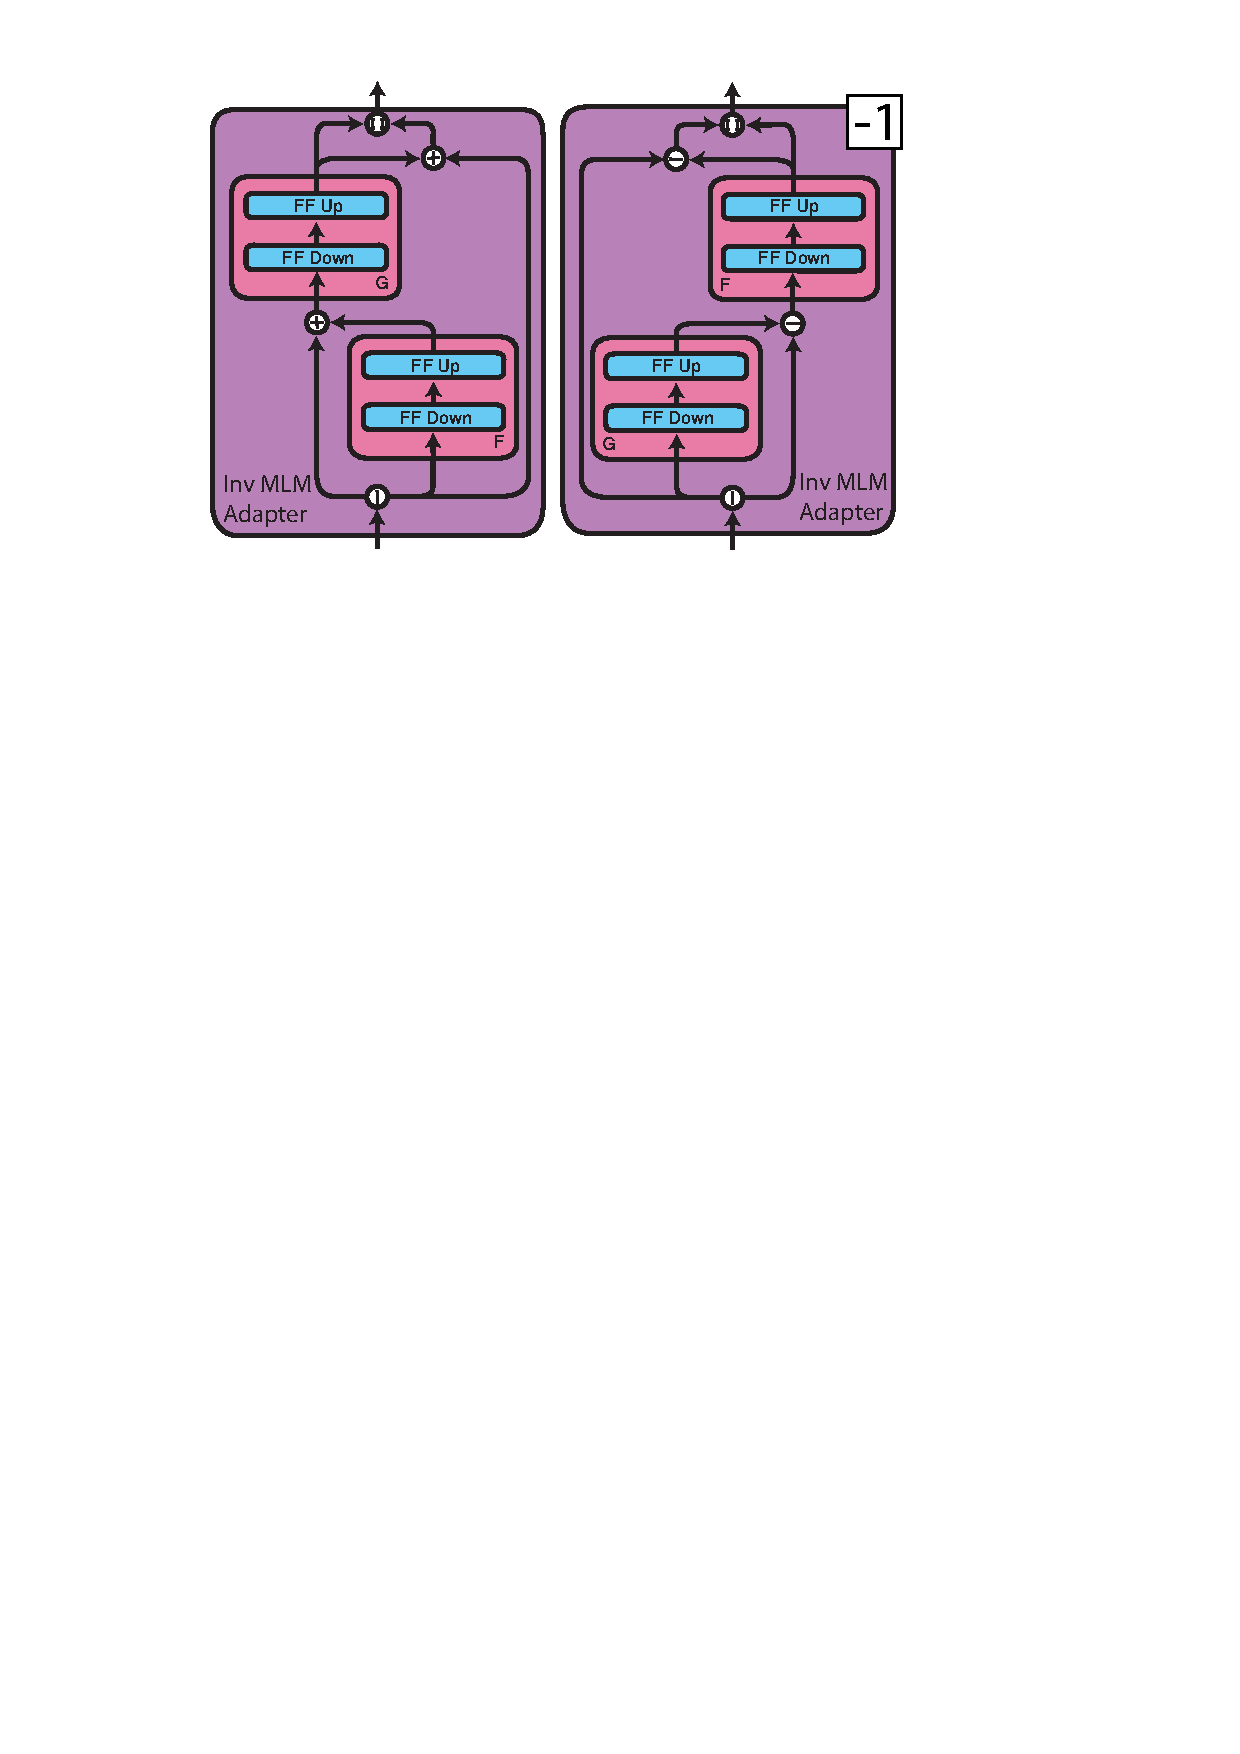
\includegraphics[width=0.6\textwidth]{figures/parameter_efficient_finetuning/MAD-X_Invertible.pdf}
    \caption{Invertible Adapter. %\TODO{better description}
    }
    \label{fig:invertible_adapter}
\end{figure}

%\mrinmaya{Can we add LoRA and Prefix tuning since there is an assignment question on it? Also, can we add some ``key'' empirical results from the various papers in all the descriptions?}

\subsection{Prefix Tuning}
Prefix tuning is another PEFT method. But different from others, it has its roots in prompting. Therefore, we will discuss it in detail in \cref{sec:prompting}. In Assignment 2, you will be asked to show how prefix tuning as well as LoRA connects to adapter tuning.
The performance of various PEFT methods are summarized in \cref{fig:peft} \citep{liu2022fewshot}. We could not cover all the methods in this course. Feel free to read their papers if you are interested.

%\TODO{Needs to be extended.}


% Other variants of adapters include prefix tuning \citep{li2021prefix}, LoRA \citep{hu2022lora}, and parallel adapter \citep[PA;][]{yu2023towards}, which are summarized in \cref{fig:adapter_other}.

% \paragraph{Prefix Tuning}

% \paragraph{LoRA} 
% \begin{equation}
%     \textbf{h}\leftarrow \textbf{h}+
% \end{equation}

% \paragraph{Parallel Adapter}

% \paragraph{Compacter}

% \paragraph{UniPELT}

% \paragraph{$(\text{IA})^3$}

% \begin{figure}[htbp]
%     \centering
%     \begin{subfigure}[t]{0.19\textwidth}
%          \centering
%          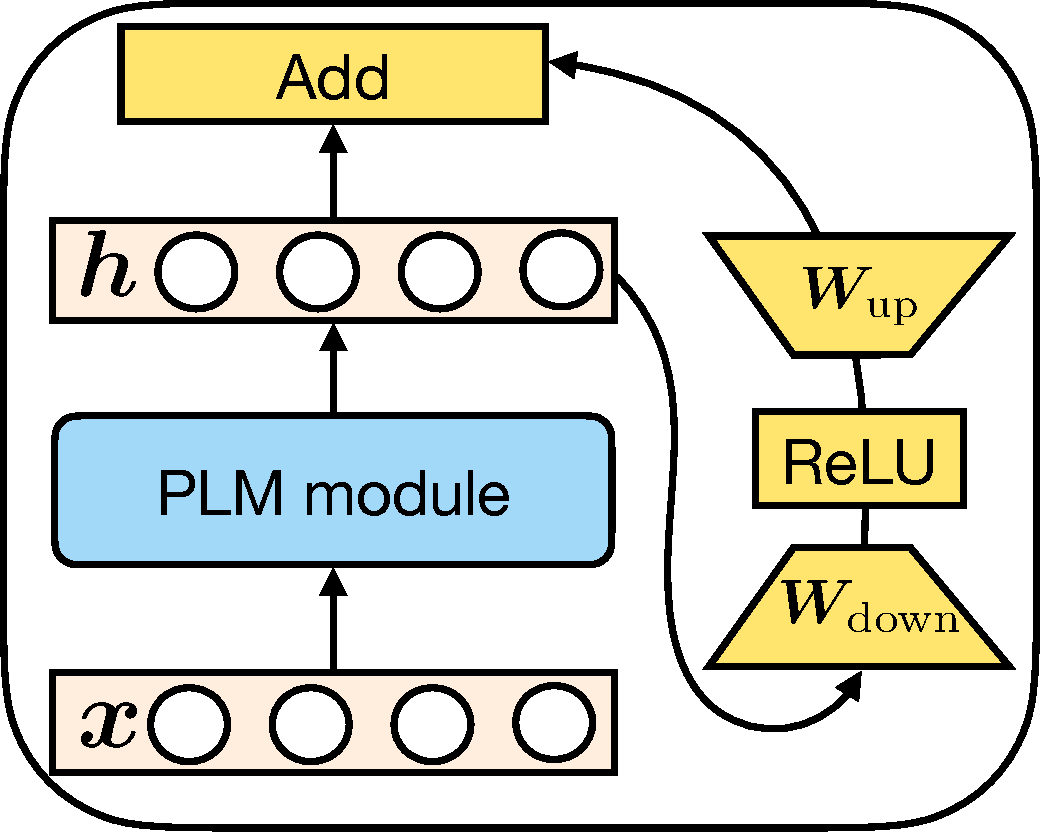
\includegraphics[width=\textwidth]{figures/parameter_efficient_finetuning/adapter.pdf}
%          \caption{Adapter}
%     \end{subfigure}
%     \hfill
%     \begin{subfigure}[t]{0.19\textwidth}
%          \centering
%          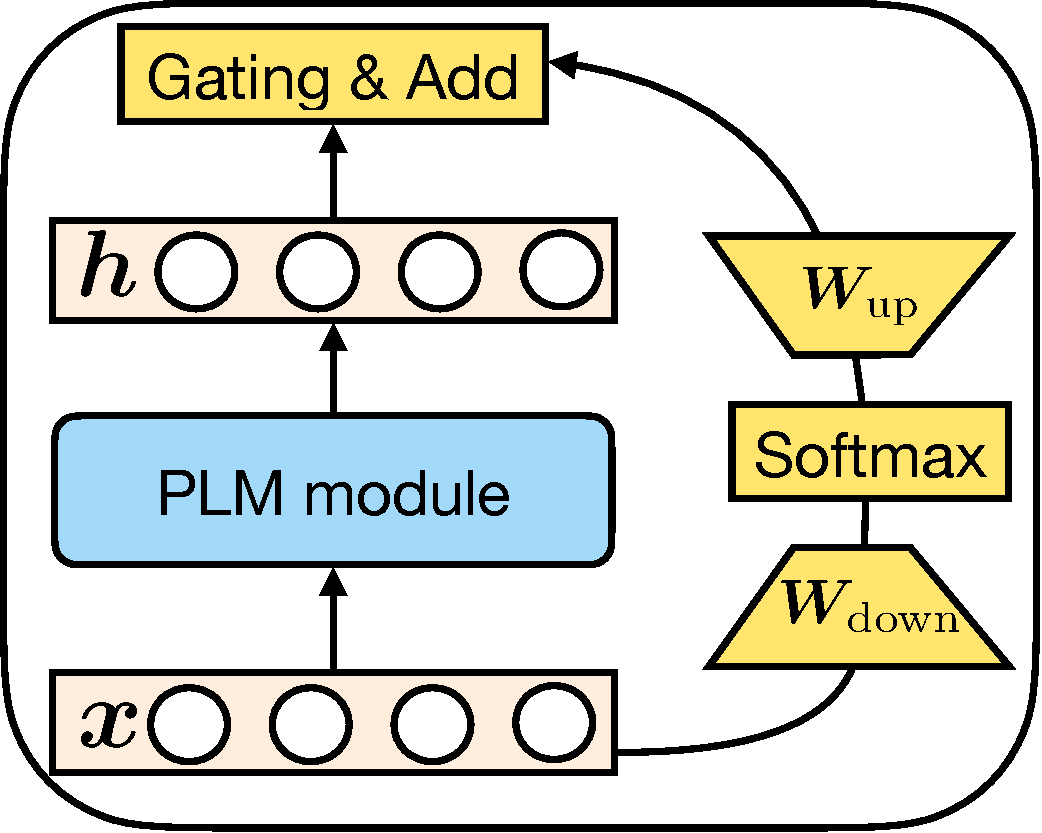
\includegraphics[width=\textwidth]{figures/parameter_efficient_finetuning/prefix.pdf}
%          \caption{Prefix Tuning}
%     \end{subfigure}
%     \begin{subfigure}[t]{0.19\textwidth}
%          \centering
%          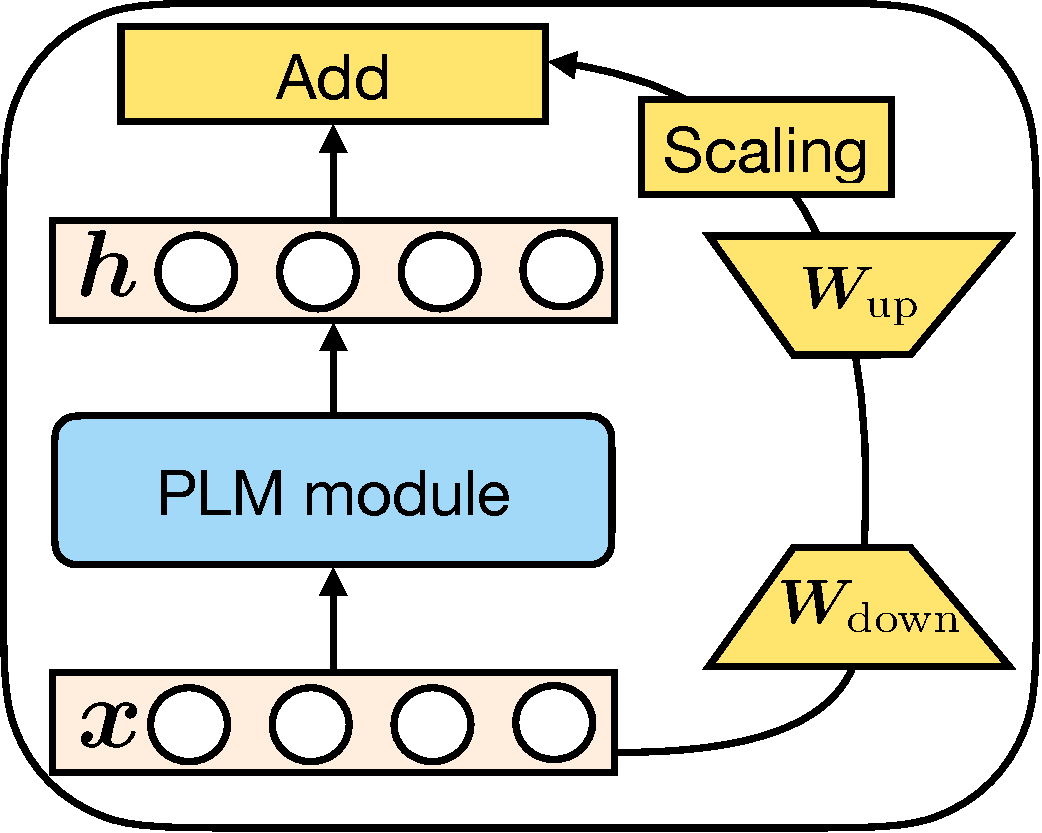
\includegraphics[width=\textwidth]{figures/parameter_efficient_finetuning/lora.pdf}
%          \caption{LoRA}
%     \end{subfigure}
%     \begin{subfigure}[t]{0.19\textwidth}
%          \centering
%          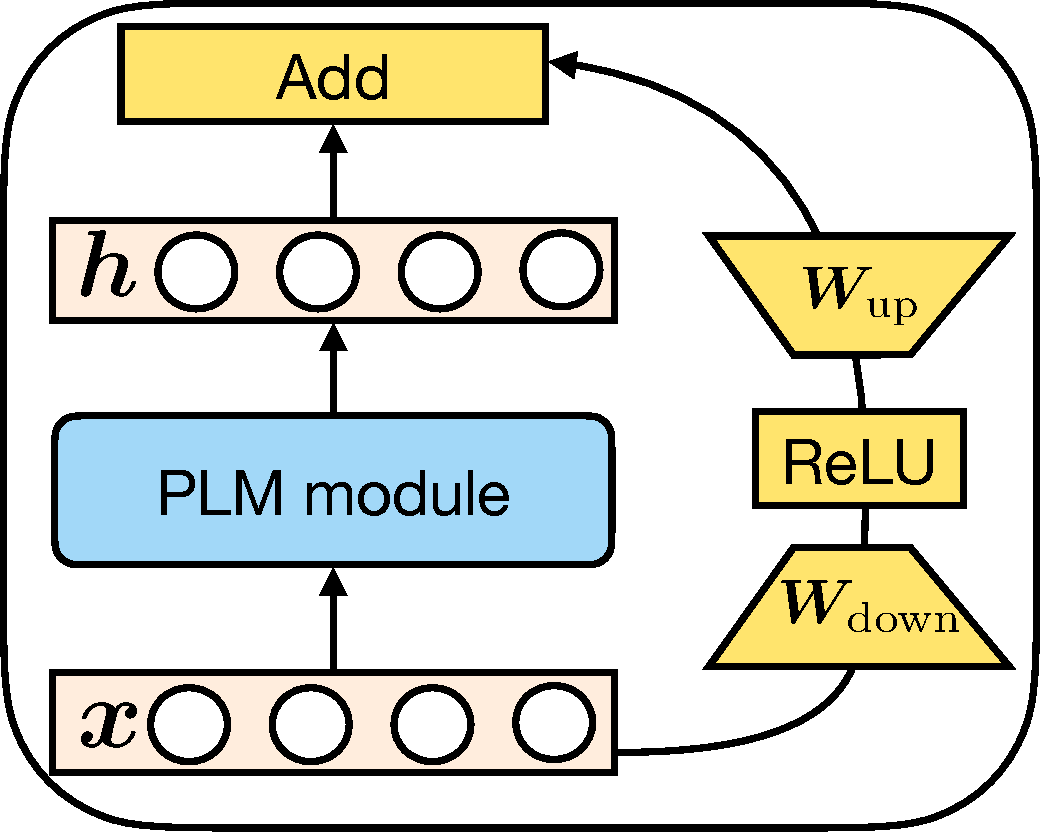
\includegraphics[width=\textwidth]{figures/parameter_efficient_finetuning/parallel.pdf}
%          \caption{Parallel Adapter}
%     \end{subfigure}
%     \begin{subfigure}[t]{0.19\textwidth}
%          \centering
%          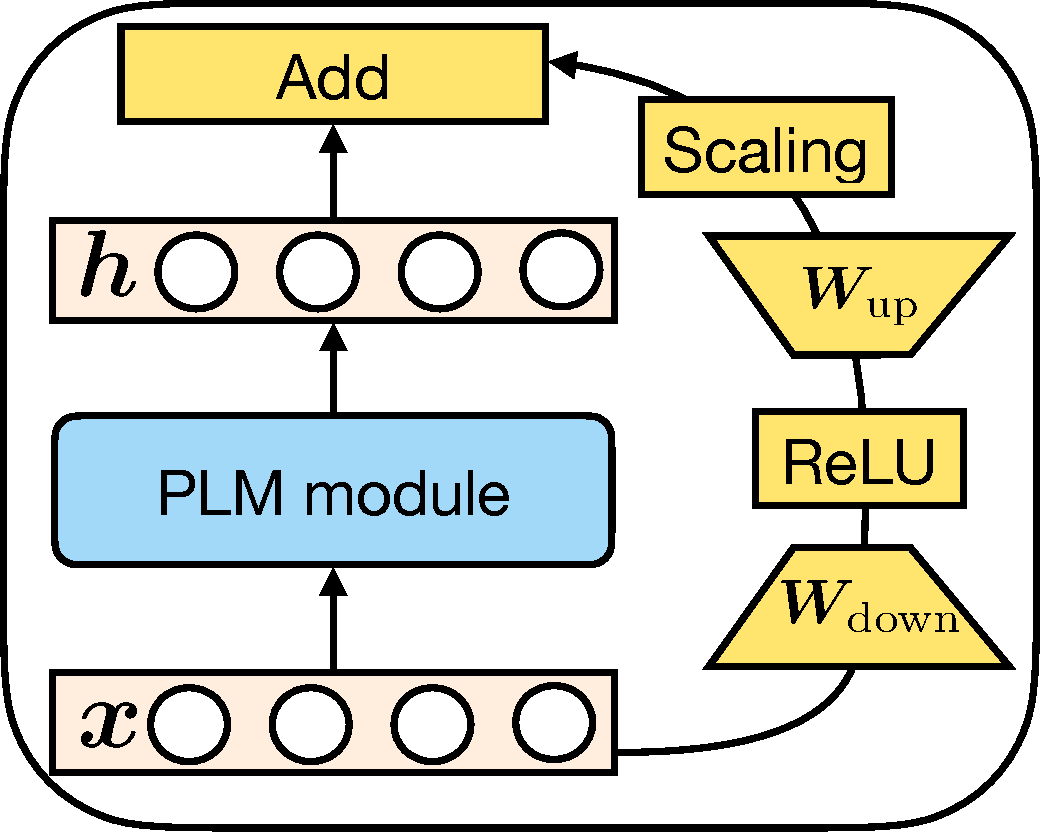
\includegraphics[width=\textwidth]{figures/parameter_efficient_finetuning/scale.pdf}
%          \caption{Scaled PA}
%     \end{subfigure}
%     \caption{Illustration of various adapter configurations.}
%     \label{fig:adapter_other}
% \end{figure}


\section{LoRA}
% \begin{figure}
%     \centering
%     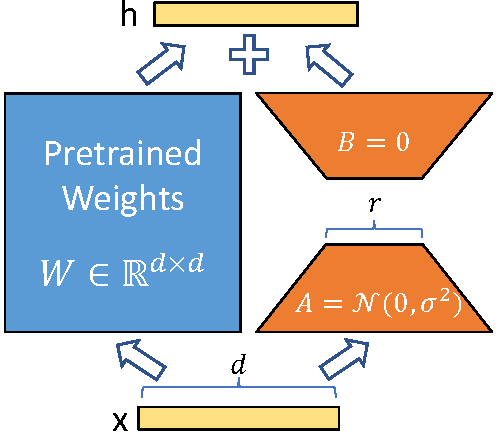
\includegraphics[width=0.5\textwidth]{figures/parameter_efficient_finetuning/figure1.pdf}
%     \caption{LoRA.}
%     \label{fig:lora}
% \end{figure}

\begin{figure}
    \centering
    \begin{minipage}{0.4\textwidth}
        \centering
        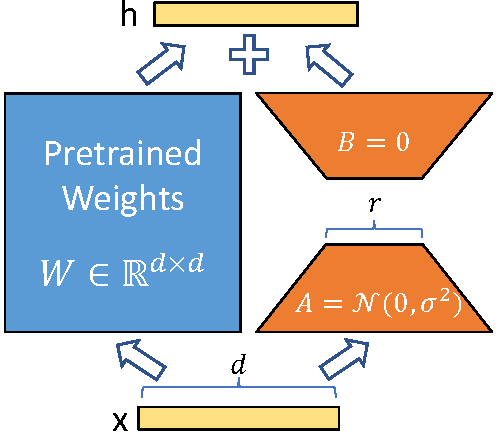
\includegraphics[width=\textwidth]{figures/parameter_efficient_finetuning/figure1.pdf}
        \caption{\textbf{LoRA}. Pretrained weight matrix $W$ is frozen during training. Inputs $x$ are transformed by $W$ to produce outputs $h$. Low-rank matrices $A$ and $B$ are trained to approximate the weight update $\Delta W$. The rank $r$ of matrices $A$ and $B$ is much smaller than the dimension $d$ of $W$, thereby reducing the number of trainable parameters and computational cost.}
        \label{fig:lora}
    \end{minipage}\hfill
    \begin{minipage}{0.4\textwidth}
        \centering
        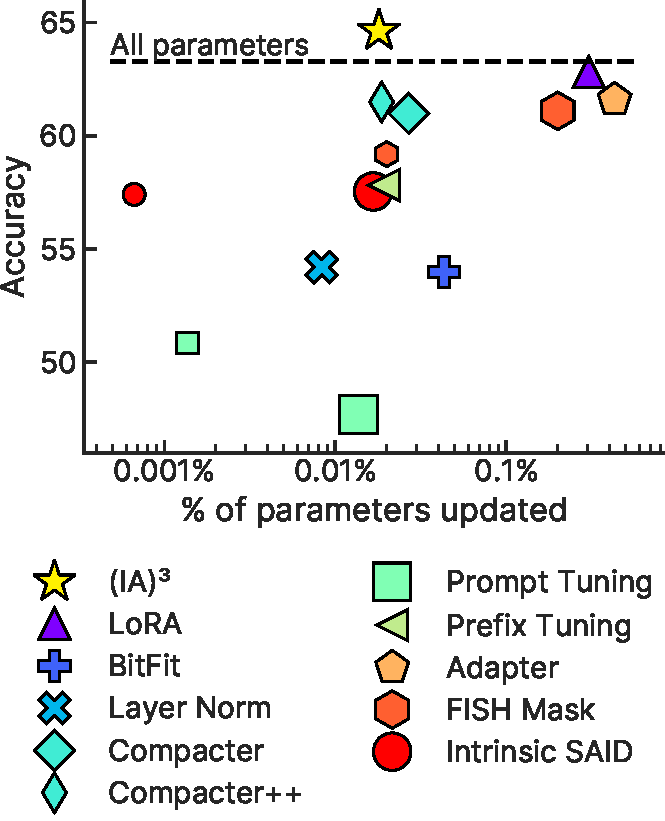
\includegraphics[width=\textwidth]{figures/parameter_efficient_finetuning/peft.pdf}
        \caption{Accuracy of PEFT methods applied to T0-3B \citep{sanh2022multitask}.}
        \label{fig:peft}
    \end{minipage}
\end{figure}


%Bottleneck adapters introduce extra compute in adapter layers, which can not be bypassed with model parallelism since they have to be processed sequentially. Even though adapter layers are designed to have very few parameters, they could still lead to a non-negligible latency, especially during inference. To address this issue, \citet{hu2022lora} propose LoRA, which injects trainable low-rank matrices to approximate the weight updates (\cref{fig:lora}). For a pre-trained weight matrix $\textbf{W}\in\mathbb{R}^{d\times k}$ (e.g., query and value projection matrices in the multi-head attentions), the update is computed with a low-rank decomposition:
%\begin{equation}
%    \Delta \textbf{W} = \textbf{B}\textbf{A}
%\end{equation}
%where $\textbf{B}\in\mathbb{R}^{d\times r}$, $\textbf{A}\in\mathbb{R}^{r\times k}$. During training, $\textbf{W}$ is frozen and only \textbf{A} and \textbf{B} are trained. \textbf{A} is initialized with a random Gaussian distribution, and \textbf{B} is initialized to be zero. The update is then scaled by a constant $\frac{\alpha}{r}$, which is roughly equivalent to tuning the learning rate. In summary, given a specific input $\textbf{x}$ to the layer, we have
%\begin{equation}
%    \textbf{h} = \textbf{W}\textbf{x} + \frac{\alpha}{r}\cdot \Delta \textbf{W}\textbf{x} = \textbf{W}\textbf{x} + \frac{\alpha}{r}\cdot \textbf{B}\textbf{A}\textbf{x}.
%\end{equation}

Bottleneck adapters, while effective in introducing task-specific adaptability into pre-trained models, come with their own set of computational challenges. One significant issue is the added computational overhead in adapter layers, which cannot be mitigated through model parallelism due to their sequential processing requirement. Although these adapters are designed to be parameter-efficient, the extra latency introduced, especially during inference, can be non-negligible and impact performance.

To tackle this bottleneck, \citet{hu2022lora} introduce the concept of Low-Rank Adaptation (LoRA), a novel approach that leverages trainable low-rank matrices to efficiently approximate weight updates in large language models (\cref{fig:lora}). LoRA specifically targets the adaptation of weight matrices $\textbf{W}\in\mathbb{R}^{d\times k}$, such as those found in the query and value projection matrices of multi-head attention mechanisms, with a low-rank decomposition strategy:
\begin{equation}
\Delta \textbf{W} = \textbf{B}\textbf{A},
\end{equation}
where $\textbf{B}\in\mathbb{R}^{d\times r}$ and $\textbf{A}\in\mathbb{R}^{r\times k}$ represent the low-rank matrices. During the training phase, the original weight matrix $\textbf{W}$ remains unchanged, while only $\textbf{A}$ and $\textbf{B}$ are updated. This method not only preserves the generalization capabilities of the pre-trained model but also significantly reduces the computational overhead associated with full model fine-tuning.

The initialization of matrix $\textbf{A}$ with a random Gaussian distribution and $\textbf{B}$ with zeros is a strategic choice that balances between maintaining the original model's performance and allowing for effective fine-tuning. Furthermore, the update to $\Delta \textbf{W}$ is scaled by a factor of $\frac{\alpha}{r}$, akin to adjusting the learning rate, which fine-tunes the extent to which these low-rank modifications influence the final model output. This scaling mechanism is crucial for controlling the fine-tuning process, ensuring that the updates enhance the model's performance on specific tasks without compromising its underlying strengths.
Given an input $\textbf{x}$ to the layer, the output $\textbf{h}$ is computed as follows:
\begin{equation}
\textbf{h} = \textbf{W}\textbf{x} + \frac{\alpha}{r}\cdot \Delta \textbf{W}\textbf{x} = \textbf{W}\textbf{x} + \frac{\alpha}{r}\cdot \textbf{B}\textbf{A}\textbf{x}.
\end{equation}
This equation encapsulates the essence of LoRA's approach: it adapts the model's behavior by adding a low-rank, trainable adjustment to the pre-existing weight matrix, enabling precise and efficient fine-tuning. By doing so, LoRA addresses the computational inefficiencies of traditional fine-tuning methods, offering a scalable solution that retains the pre-trained model's robustness while customizing it for specific tasks or datasets.

\subsection{Advantages}
The LoRA method boasts several compelling advantages that make it particularly attractive for fine-tuning large language models. Notably, its efficiency is a standout feature. By adjusting only a fraction of the model's parameters through low-rank matrices, LoRA dramatically reduces the computational burden typically associated with fine-tuning. This efficiency does not come at the cost of performance; empirical results have demonstrated that LoRA can match or even exceed the performance of traditional fine-tuning techniques on downstream tasks.

Another significant advantage of LoRA is its flexibility. The method is not prescriptive about which parts of the transformer model it can be applied to. This means that practitioners can apply LoRA to the specific parts of the model that most impact the task at hand, whether that be attention mechanisms, feed-forward networks, or other components. This flexibility allows for a targeted approach to fine-tuning, ensuring that the adaptations made to the model are directly relevant to the improvements sought.

Moreover, despite the reduced number of trainable parameters, LoRA maintains—or in some cases, enhances—the model's capacity for generalization. This characteristic is particularly important when applying fine-tuned models to a range of scenarios or datasets that may differ from the data used during training. By striking a balance between efficiency, flexibility, and performance, LoRA emerges as a method well-suited to the evolving demands of natural language processing tasks and the fine-tuning of state-of-the-art language models.

% \begin{figure}[htbp]
%     \centering
%     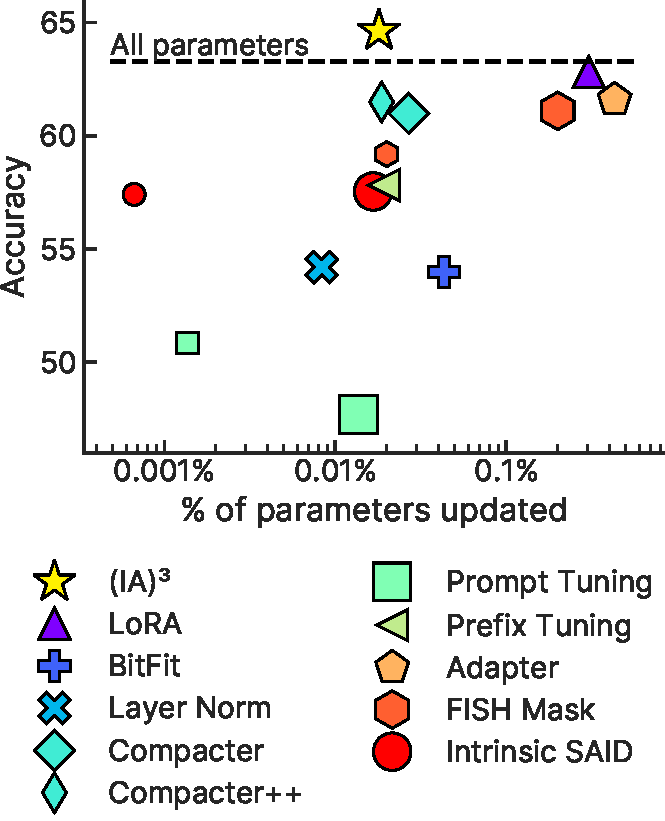
\includegraphics[width=0.5\textwidth]{figures/parameter_efficient_finetuning/peft.pdf}
%     \caption{Accuracy of PEFT methods applied to T0-3B \citep{sanh2022multitask}.}
%     \label{fig:peft}
% \end{figure}

